% 图 2：状态变量图 / 模拟结构图（n 个积分通道）
\documentclass[border=6pt]{standalone}
% 四张示意图共用的字体、颜色与 TikZ 设置
\usepackage{fontspec}
\usepackage{xeCJK}
\setmainfont{TeX Gyre Pagella}
\setCJKmainfont{Noto Serif CJK SC}[AutoFakeSlant=0.15]
\usepackage{unicode-math}
\setmathfont{TeX Gyre Pagella Math}
\usepackage{amsmath}
\usepackage{tikz}
\usetikzlibrary{arrows.meta, positioning, calc, decorations.markings, backgrounds, fit, shapes.geometric}

\definecolor{navy}{HTML}{1E3A8A}
\definecolor{teal}{HTML}{0F766E}
\definecolor{amber}{HTML}{B45309}
\definecolor{softblue}{HTML}{EFF6FF}
\definecolor{softteal}{HTML}{F0FDFA}
\definecolor{softamber}{HTML}{FFFBEB}
\definecolor{border}{HTML}{CBD5E1}
\definecolor{graytext}{HTML}{5B6673}
\definecolor{redalert}{HTML}{991B1B}

\tikzset{
  >=Latex,
  every node/.style={font=\small},
  block/.style={draw=navy, thick, rounded corners=3pt, fill=softblue, align=center},
  bus/.style={thick, graytext},
}

\begin{document}
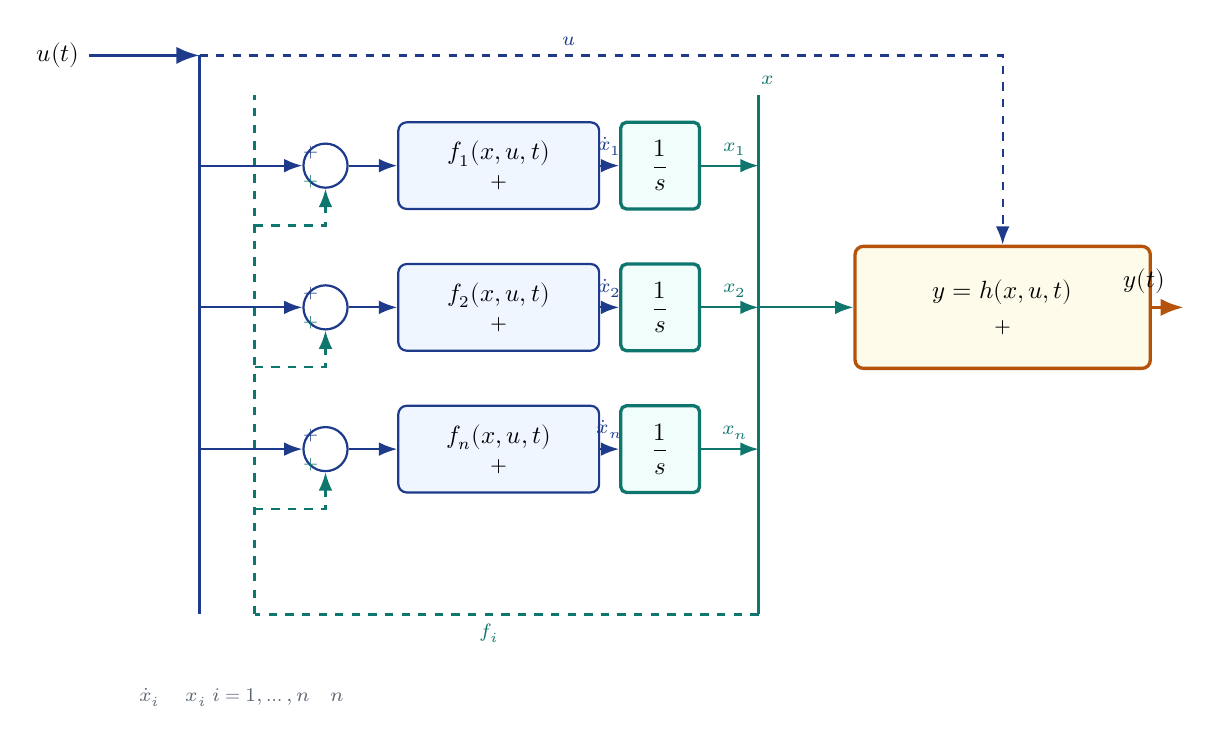
\begin{tikzpicture}[x=1cm,y=1cm]
  % 行坐标
  \def\yA{4.2}
  \def\yB{2.4}
  \def\yC{0.6}

  % 输入源与输入总线
  \node[anchor=east] (usrc) at (-1.25,5.6) {$u(t)$};
  \draw[->, very thick, navy] (usrc.east) -- (0.15,5.6);
  \draw[very thick, navy] (0.15,5.6) -- (0.15,-1.5);

  % 状态反馈总线（左侧虚线）
  \draw[very thick, teal, dashed] (0.85,-1.5) -- (0.85,5.1);
  \node[text=teal, font=\scriptsize, anchor=west] at (0.15,-1.95)
        {状态反馈总线（虚线）};

  % 三条通道
  \foreach \y/\lab in {\yA/1,\yB/2,\yC/n}{
    % 求和点
    \node[circle, draw=navy, thick, fill=white, minimum size=0.56cm] (sum\lab) at (1.75,\y) {};
    \node[text=navy, font=\scriptsize] at (1.56,\y+0.17) {$+$};
    \node[text=teal, font=\scriptsize] at (1.56,\y-0.20) {$+$};
    \draw[->, thick, navy] (0.15,\y) -- (sum\lab.west);

    % f_i 加法器 / 比例器
    \node[block, minimum width=2.55cm, minimum height=1.10cm] (f\lab) at (3.95,\y)
      {$f_{\lab}(x,u,t)$\\[-1pt]{\scriptsize 加法器 + 比例器}};
    \draw[->, thick, navy] (sum\lab.east) -- (f\lab.west);

    % 积分器
    \node[draw=teal, very thick, rounded corners=2pt, fill=softteal,
          minimum width=1.0cm, minimum height=1.10cm] (int\lab) at (6.0,\y)
          {$\dfrac{1}{s}$};
    \draw[->, thick, navy] (f\lab.east) -- node[above, font=\scriptsize] {$\dot x_{\lab}$} (int\lab.west);
    \draw[->, thick, teal] (int\lab.east) -- (7.25,\y);
    \node[above, text=teal, font=\scriptsize] at (6.95,\y) {$x_{\lab}$};

    % 状态反馈支路：从左侧状态总线进入求和点下方
    \draw[->, thick, teal, dashed] (0.85,\y-0.76) -- (1.75,\y-0.76) -- (sum\lab.south);
  }

  % 状态收集总线
  \draw[very thick, teal] (7.25,-1.5) -- (7.25,5.1);
  \node[above, text=teal, font=\scriptsize] at (7.25,5.1) {状态 $x$};
  % 反馈总线回到左侧
  \draw[thick, teal, dashed] (7.25,-1.5) -- (0.85,-1.5);
  \node[below, text=teal, font=\scriptsize] at (4.0,-1.5)
        {每个 $f_i$ 可依赖全部状态};

  % 输出映射 h
  \node[draw=amber, very thick, rounded corners=3pt, fill=softamber, align=center,
        minimum width=3.75cm, minimum height=1.55cm] (h) at (10.35,2.4)
        {$y=h(x,u,t)$\\[1pt]{\scriptsize 加法器 + 比例器}};
  \draw[->, thick, teal] (7.25,2.4) -- (h.west);
  % u 也进入 h（沿顶部走线）
  \draw[->, thick, navy, dashed] (0.15,5.6) -- (10.35,5.6) -- (h.north);
  \node[above, text=navy, font=\scriptsize] at (5.1,5.6) {$u$ 进入输出映射};
  \draw[->, very thick, amber] (h.east) -- (12.65,2.4);
  \node[above] at (12.15,2.45) {$y(t)$};

  % 说明
  \node[text=graytext, anchor=west, align=left, font=\scriptsize] at (-1.25,-2.55)
    {每个积分器把 $\dot x_i$ 变成 $x_i$；$i=1,\dots,n$ 共 $n$ 路。};
\end{tikzpicture}
\end{document}
